\documentclass[10pt,twocolumn,letterpage]{article}
\usepackage{times,amsmath,amsfonts, bm, empheq, graphicx}
%\usepackage[dvips]{graphicx,graphics}
\usepackage{subfig}
\usepackage{titlesec}
\usepackage{float}

\titleformat{\section}{\Large\bfseries\filcenter}{\thesection.}{0.2em}{}
\titleformat{\subsection}{\large\bfseries\filright}{\thesubsection}{0.5em}{}
\titleformat{\subsubsection}{\normalsize\bfseries\filright}{\thesubsubsection}{0.5em}{}
\titlespacing{\section}{0pt}{3ex plus 0.5ex minus 0.2ex}{2ex plus .2ex}
\titlespacing{\subsubsection}{0pt}{2ex plus 0.1ex minus 0.1ex}{1ex plus .2ex}
\graphicspath{{figures/}}


% \titleformat{command}[shape]{format}{label}{sep}{beforecode}[aftercode]
% \fontsize{size}{baseline skip}

\setlength{\textheight}{8.5in} \setlength{\textwidth}{5.5in}
\setlength{\headheight}{0in} \setlength{\headsep}{0in}
\setlength{\parindent}{1pc}
\setlength{\parskip}{0pc}
\setlength{\oddsidemargin}{0.3in} 
\setlength{\evensidemargin}{0in}
\setlength{\columnsep}{1.5em}




\begin{document}
	\title{\textbf{Sentimental Analysis of IMDb Movie Reviews}}
	\author{Haoming Chen\\
		{\tt\small hchen549@wisc.edu}
		\and
		Ruiting Tong\\
		{\tt\small rtong5@wisc.edu}
		\and
		Dingyi Li\\
		{\tt\small dli283@wisc.edu}
	}
	\date{}
	\maketitle

		\section*{Abstract} 
			\textit{The objective of this project is to predict sentimental representation from the review of movies listed on IMDb via several classification machine learning algorithms. We collected 50,000 movie reviews and their sentiment scores (0 and 1) and processed them for analysis. The data are divided into 70\% of training set and 30\% of test set. Algorithms of SVM, KNN, Decision Tree, Logistic Regression, and Random Forest are trained and tested for accuracy. In particular, we used both the RBF and the linear kernels for SVM, and we applied bagging to Logistic Regression to obtain and verify an increased accuracy. As a result, we have found that the Logistic Regression is the best option for this task among others.} 			

		\section{Introduction} 
			 With the Internet and modern technology, people are able to produce tons of text data every single day. We can find such data in emails, comments on articles, reviews on products, and social media, and there is a lot of information contained within such text data. When people write things down, they are motivated by certain emotions or attitudes. If they were happy with a product or an experience, they would compliment it and recommend it to others. If they had a terrible experience, they would criticize it and caution others. If we are able to organize and analyze the text data in a way that could accurately reflect users’ emotion or attitude, which is referred to as sentimental analysis, the companies could modify the service provided to each individual accordingly.
			 
			 Internet Movie Database (IMDb) is one of the most popular online databases for movies where millions of users read and write movie reviews. The users’ attitude toward one movie could be inferred by looking at the reviews they made. In this project, we consider the simplest case where the sentiment is represented by a binary indicator: 1 meaning positive and 0 meaning negative. Despite such a simplification, it would be impossible for humans to read through millions of comments and reviews made by all movie watchers and label them each with a sentiment score. Therefore, it is necessary that we train and implement a machine learning algorithm to accomplish this task in our place. 
			 
			 Solving this classification problem is the first step to uncover the underlying habits of different users. One of the beneficiaries of such analysis would be streaming sites such as Netflix that need such data and methods to find out the movie types that particularly interest each user, and make accurate recommendations. On top of that, they can filter some junk ratings that are not conducive to helping others correctly understand and evaluate a movie, since they can be purely emotional and not based on reasons. 
			 
			 To find out the most suitable classification algorithm for this task, we experiment with SVM (RBF and linear kernels), KNN, Decision Tree, Random Forest, and Logistic Regression (with and without bagging). First of all, we extract 50,000 movie reviews and their corresponding 0-1 labels, and clean up the data by \textit{Natural Language Toolkit} (NLTK) package of Python. Then, we use 70\% of the data for training and the rest for testing. All the aforementioned algorithms are trained using the features selected in the first step. Lastly, test accuracy is computed for each algorithm, and further analyses such as McNemar's test and ROC comparisons are implemented to rank the algorithms.
		\section{Proposed Methods}
		\subsection{Support Vector Machine}
			Support Vector Machine (SVM) is a very commonly used algorithm for binary classification. The motivation behind it is relatively easy to understand. Basically, in an n-dimensional feature space, we want to find a (n-1)-dimensional hyperplane that separates the datapoints of two different classes, assuming that they are indeed separable by a line. Suppose that the hyperplane is $$\bm{\omega}^\top \bm{x} + b = 0.$$ and that \begin{equation}
				\bm{\omega}^\top \bm{x} + b = \pm1 \label{hyp}
			\end{equation} happen to be boundaries of the two classes that touch on at least one sample from each class respectively. Our goal is then to maximize the distance between the two hyperplanes in \ref{hyp}. Such a distance is given by $$\frac{2}{||\bm{\omega}||},$$ which can be interpreted as the distance between the two classes. The optimal hyperplane obtained from solving this maximization problem is used for prediction of new data. 
			
			So far, the idea of SVM has been introduced for the linear kernel. In fact, we can replace $\bm{x}$ in the constraint to an arbitrary function $\phi(\bm{x})$. Then the separating surface may no longer be a hyperplane. For example, a nonlinear kernel $\kappa(\bm{x},\bm{y}) = \phi(\bm{x})^\top \phi(\bm{y})$ that we have also employed is the Radial Basis Function (RBF), which is given by $$\kappa(\bm{x},\bm{y}) = \exp\left(-\frac{||\bm{x}-\bm{y}||^2}{2\sigma^2}\right),$$ where $||\cdot||$ denotes the Euclidean distance and $\sigma$ represents the bandwidth.  
			
			$L_1$ regularization is applied to SVM with linear kernel, and the coefficient $c$ is tuned. 
		\subsection{k Nearest Neighbors}
			$k$ Nearest Neighbors (KNN) is a classification algorithm whose training step only involves remembering the data. Suppose the size of the training set is $N$. In the fitting step, for each new sample $x^*$, the algorithm computes $$d_i = ||x^* - x_{\text{train},i}|| \text{ for } i = 1,2,...,N,$$ where $||\cdot||$ can be any distance function. Then we pick the $k$ indices from $\{1,2,...,N\}$ that are associated with the $k$ smallest distances. The predicted label for $x^*$ is the majority vote of the labels corresponding to these indices. 
			
			For our problem, we only consider the Euclidean distance, and $k$ is the only parameter we need to tune for. Considering that the optimal $k$ could be very large given a very high-dimensional data set, we search for such $k$ manually by narrowing down the search range.
		\subsection{Decision Tree}
			A decision tree predicts the label of a new sample by searching for the leaf node it belongs to. A tree can be either binary or non-binary, the information criterion for splitting a node can be "Gini", "Entropy", and so on, and the maximum depth is yet another hyperparameter that is set to prevent overfitting. In our project, we require the tree to be binary, while letting information criterion and maximum depth be unknown hyperparameters to optimize. Similar to the $k$ in $k$ Nearest Neighbors algorithm, the maximum depth is not searched for exhaustively. It is pinpointed by manually narrowing the search range.
		\subsection{Random Forest}
			Random Forest is an ensemble method augmented from decision trees. In our case, 100 trees are being trained, and at each node, a random set of features are chosen for the purpose of splitting. The prediction is the majority vote of the 100 trees. Notice that we do not perform any hyperparameter tuning for random forest for the sake of runtime. The maximum depth is set to "None" and the criterion is fixed as "Entropy".
		\subsection{Logistic Regression}
			Unlike the previous algorithms, the logistic regression is a soft classifier that predicts the conditional probability of a label being 0 or 1. Explicitly, 
			$$P(y = 0) = \frac{1}{1+\exp(\bm{\beta^\top}\bm{x})},$$ where $\bm{\beta}$ is estimated from the training set by minimizing \begin{align*}
				&-2\log L(\bm{X_1},...,\bm{X_N}) \\
				&= -2\log (\prod_{i=1}^{N}P_i^{1-Y_i}(1-P_i)^{Y_i})\\
				&= -2\sum_{i=1}^{N}(Y_i\bm{\beta}^\top\bm{X_i} - \log(1+\exp(\bm{\beta}^\top\bm{X_i}))).
			\end{align*} 
			However, in order to avoid overfitting, we add an $L_1$ regularization term to the cost function. Its coefficient is $c$, which is a hyperparameter we need to optimize.
		\subsection{Bagging}
			Bagging is an ensemble method to improve the performance of an algorithm. In our project, we only apply it to the logistic regression. This seemingly arbitrary decision is made not only because the logistic regression has a high test accuracy to be worthy of a further uplift, but also because it is the fastest algorithm among others so as to make bagging very applicable. The $L_1$ regularization coefficient is inherited from the regular logistic regression. 
			
			Different bagging sizes are attempted to help us visualize a pattern of increase in test accuracy. 
		\section{Experiment}	
		\subsection{Language Processing}
		\subsubsection{Removing HTML tags, special characters, and stop words}
		Being read the internet, raw review data contains tags that constitute the grammar of HTML, punctuation, and words that are not related to sentiments (stop words). We remove these irrelevant components: 
			
			\begin{figure}[htbp]
				\textsf{Before:}
				
				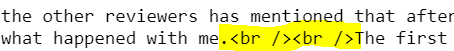
\includegraphics[width = \columnwidth]{html_tag}
				\textsf{After:}
				
				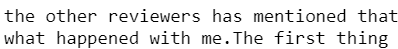
\includegraphics[width = \columnwidth]{html_tag_removed}
				\caption{Removal of HTML tags}
			\end{figure}
	
			\begin{figure}[htbp]
				\textsf{Before:}
				
				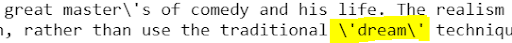
\includegraphics[width = \columnwidth]{special_char}
				\textsf{After:}
				
				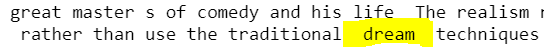
\includegraphics[width = \columnwidth]{special_char_removed}
				\caption{Removal of special characters}
			\end{figure}
	
			\begin{figure}[htbp]
				\textsf{Before:}
			
				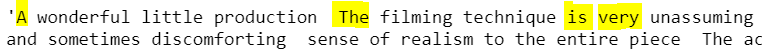
\includegraphics[width = \columnwidth]{stop_words}
				\textsf{After:}
			
				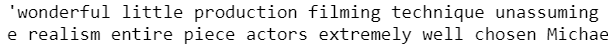
\includegraphics[width = \columnwidth]{stop_words_removed}
				\caption{Removal of stop words}
			\end{figure}
		\subsubsection{Text Stemming}
			Words such as "go" and "went" do not make essential difference. They are only different due to the English grammar. We therefore stem the text to coerce such words into one and the same feature:
			\begin{figure}[H]
				\textsf{Before:}
			
				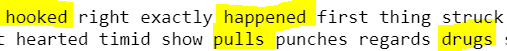
\includegraphics[width = \columnwidth]{stem}
				\textsf{After:}
			
				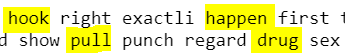
\includegraphics[width = \columnwidth]{after_stem}
				\caption{Text Stemming}
			\end{figure}

		\subsubsection{Vectorization}
			Now we need to turn features (words) into a design matrix. This step is performed by the \textit{CountVectorizer} class imported from \textit{sklearn}. A total of 70847 features are extracted.
			\begin{figure}[H]
				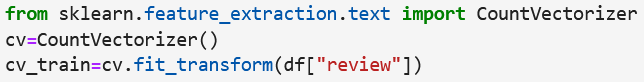
\includegraphics[width = \columnwidth]{vectorization}
				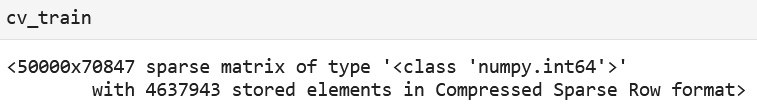
\includegraphics[width = \columnwidth]{vec_result}
				\caption{The code and result for vectorizing reviews}
			\end{figure}
	
		\subsection{Model Training}
			The dataset is divided into 70\% of training data and 30\% of test data. The split is stratified by the labels to guarantee that the training and the test sets contain homogeneous features. A random seed of 1 is used whenever randomness is involved. Hyperparameter tuning, when there are hypermarameters in an algorithm, is conducted by cross validation with k set to 5. 
		\subsubsection{SVM with RBF kernel}
\end{document}